\begin{figure}
     \centering
     \begin{subfigure}[b]{0.49\textwidth}
         \centering
         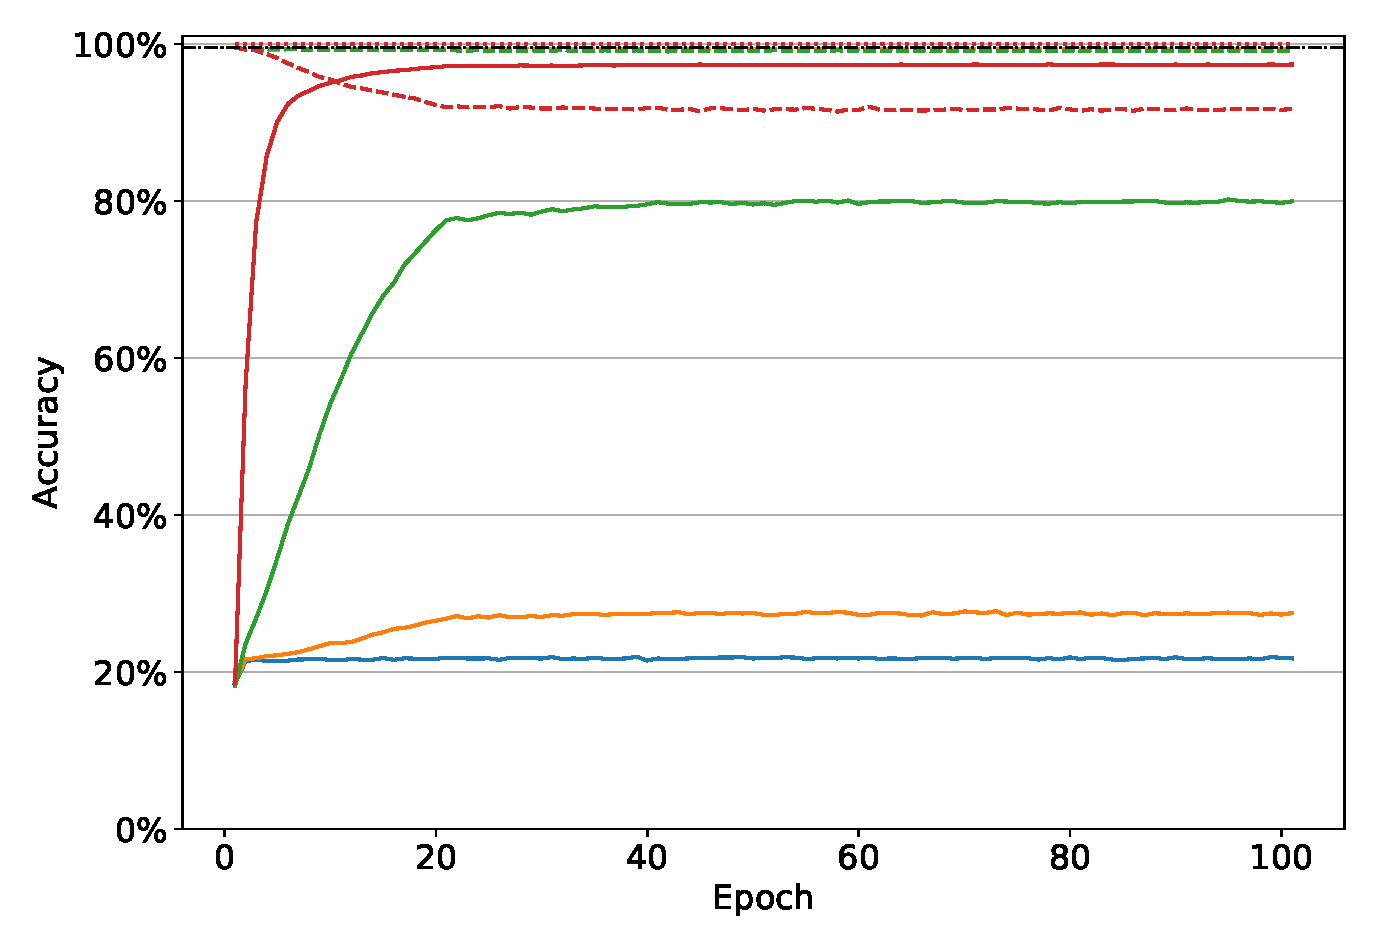
\includegraphics[width=\textwidth]{images/finetuning/finetuning_protecting_content_smalllr_thesis_simplenet_mnist.eps}
         \caption{SimpleNet, small learning rates (MNIST)}
         \label{fig:finetuning_simplenet_smalllr}
     \end{subfigure}
     \hfill
     \begin{subfigure}[b]{0.49\textwidth}
         \centering
         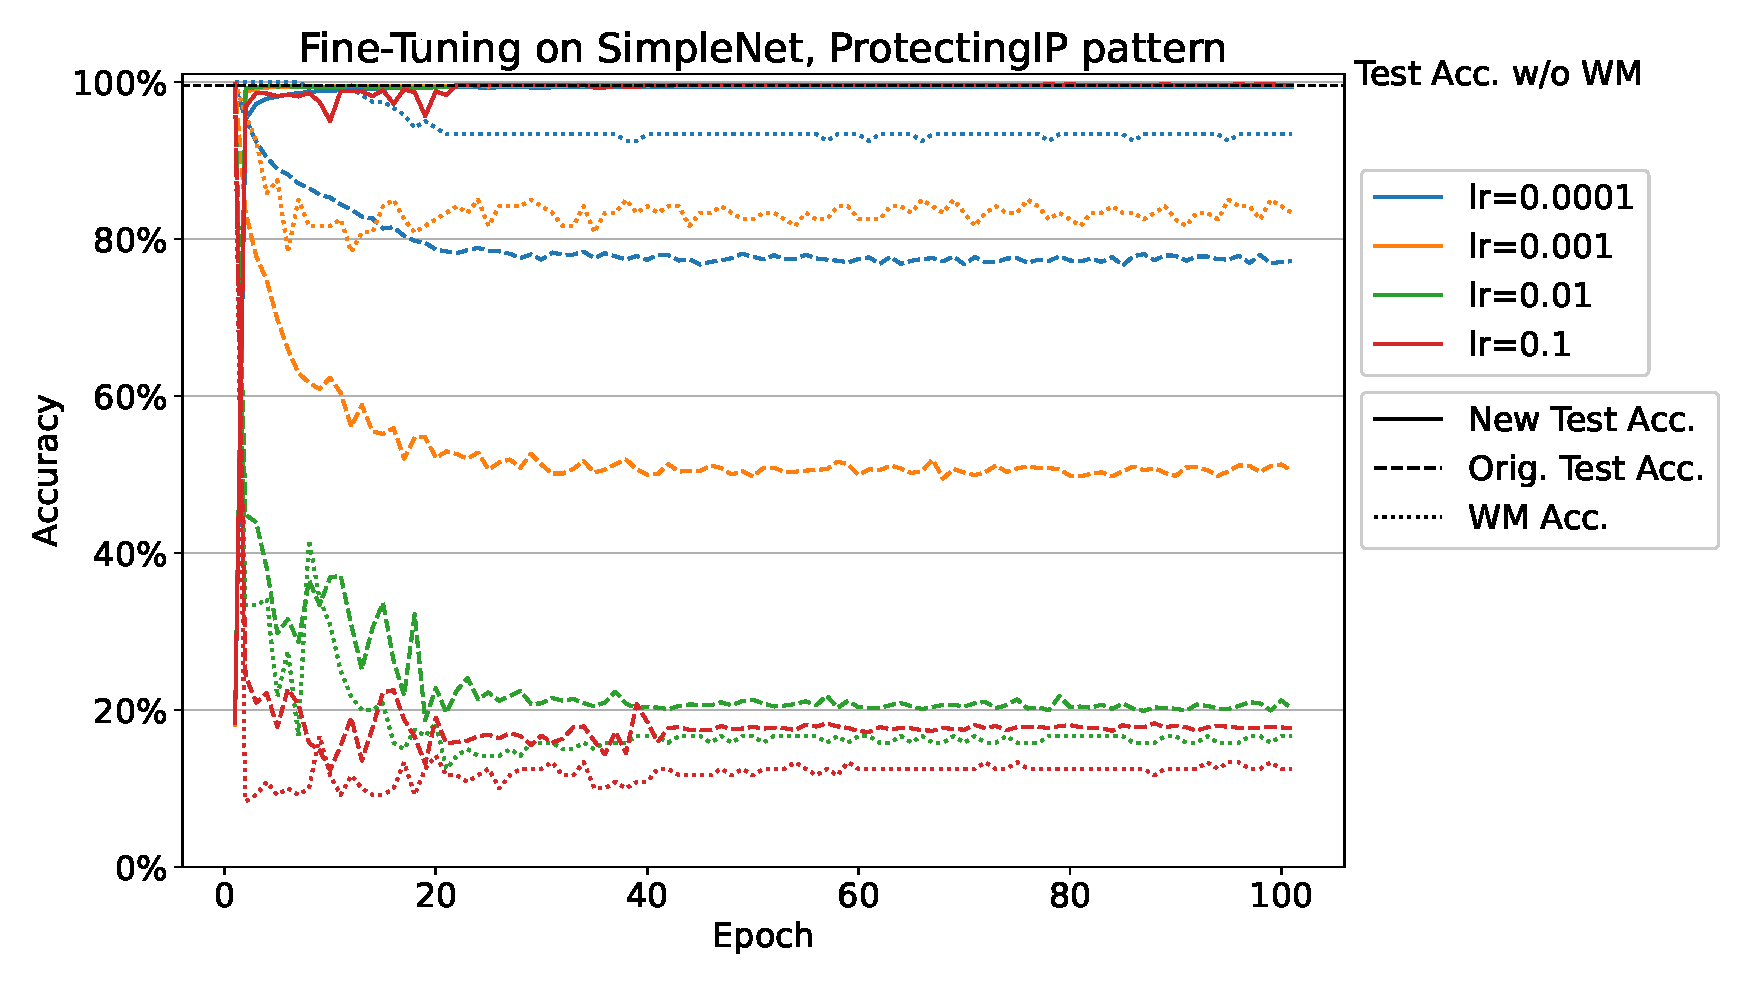
\includegraphics[width=\textwidth]{images/finetuning/finetuning_protecting_content_largelr_thesis_simplenet_mnist.eps}
         \caption{SimpleNet, large learning rates (MNIST)}
         \label{fig:finetuning_simplenet_largelr}
     \end{subfigure}
     \hfill
     \begin{subfigure}[b]{0.49\textwidth}
         \centering
         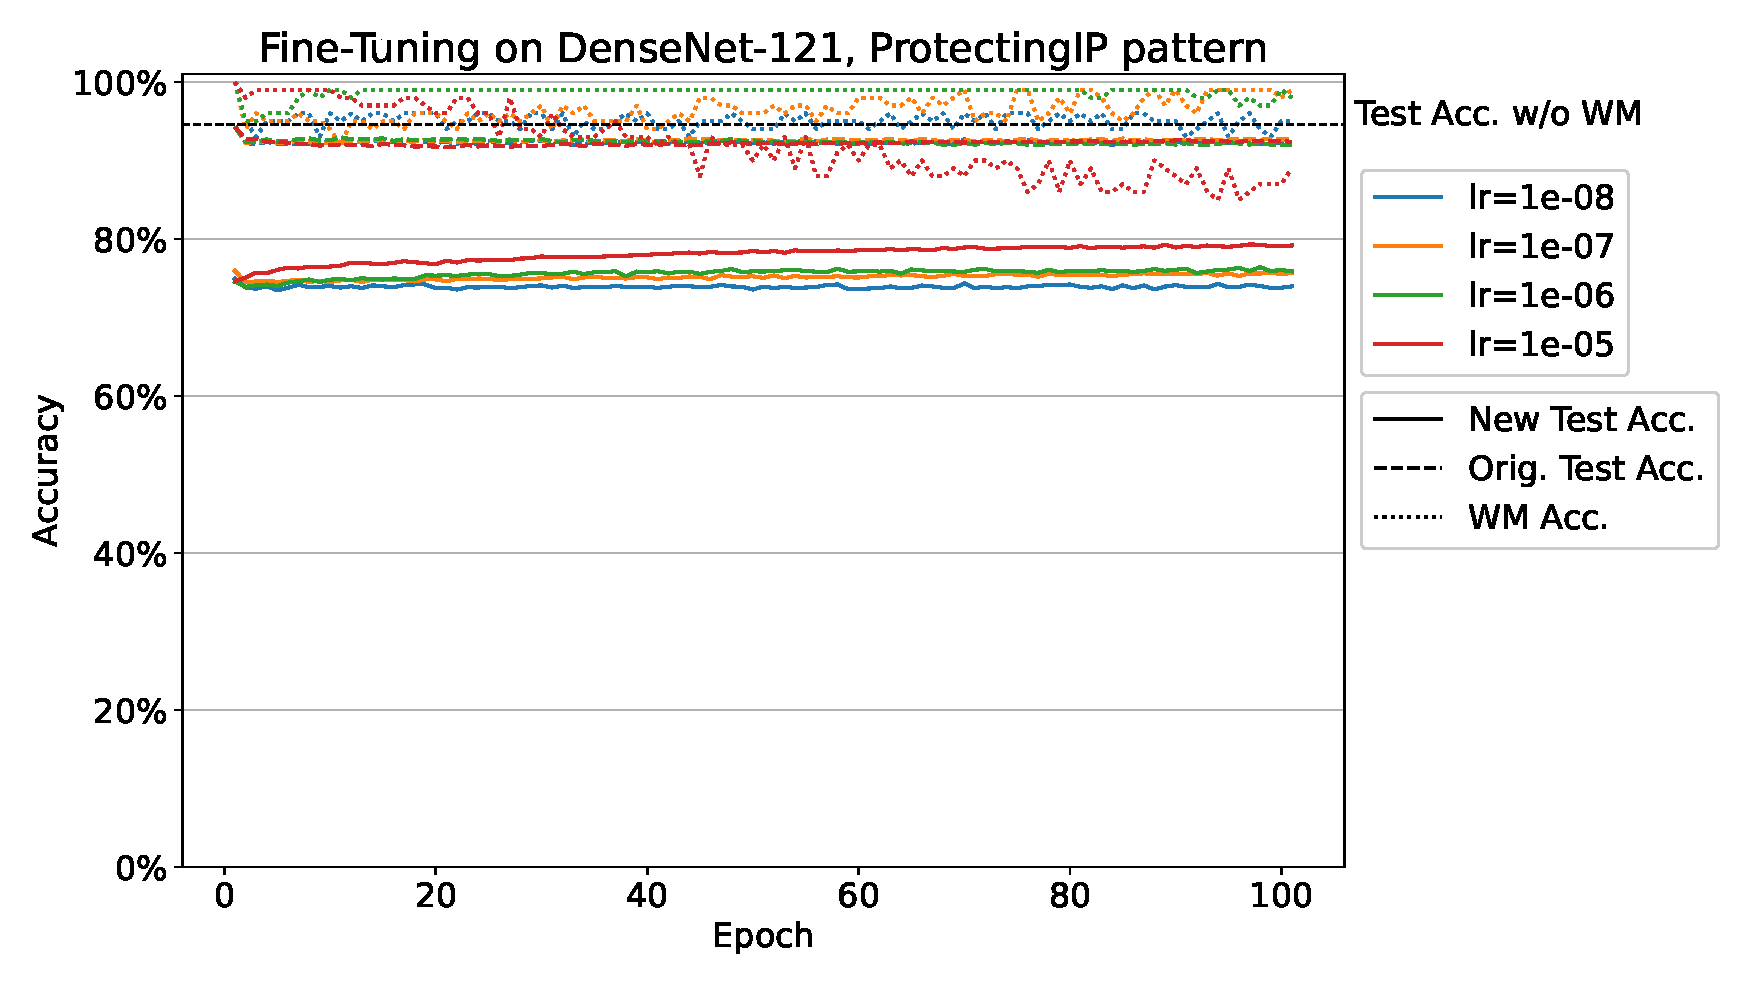
\includegraphics[width=\textwidth]{images/finetuning/finetuning_protecting_content_smalllr_thesis_densenet.eps}
         \caption{DenseNet, small learning rates (CIFAR-10)}
         \label{fig:finetuning_densenet_smalllr}
     \end{subfigure}
     \hfill
     \begin{subfigure}[b]{0.49\textwidth}
         \centering
         \includegraphics[width=\textwidth]{images/finetuning/finetuning_protecting_content_largelr_thesis_densenet.eps}
         \caption{DenseNet, large learning rates (CIFAR-10)}
         \label{fig:finetuning_densenet_largelr}
     \end{subfigure}
     \hfill
     \begin{subfigure}[b]{\textwidth}
         \centering
         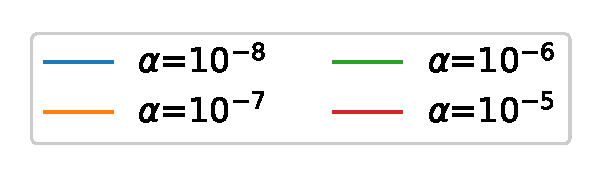
\includegraphics[height=1.1cm]{images/finetuning/legend_content_finetuning_smalllr_colors.eps}
         \quad
         \includegraphics[height=1.3cm]{images/finetuning/legend_content_finetuning_linetypes.eps}
         \quad
         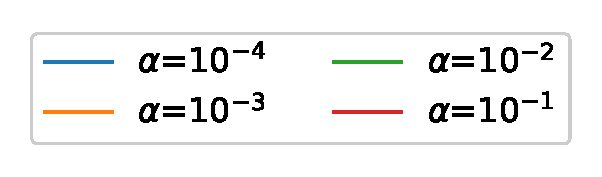
\includegraphics[height=1.1cm]{images/finetuning/legend_content_finetuning_largelr_colors.eps}
     \end{subfigure}
     \caption{Fine-tuning on SimpleNet and DenseNet, watermarked with ProtectingIP-pattern. The plots on the left side correspond to fine-tuning with smaller learning rates and the ones on the right side to fine-tuning with larger learning rates. The black dash-dotted line corresponds to the benchmark test accuracy of the non-watermarked model.}
     
     \label{fig:finetuning_simplenet_and_densenet}
\end{figure}